\documentclass[tikz,border=2mm]{standalone}
\usepackage{tikz}
\usetikzlibrary{shapes.geometric,arrows.meta,positioning,fit,patterns,calc,shadows,decorations.text,decorations.pathmorphing}

\begin{document}
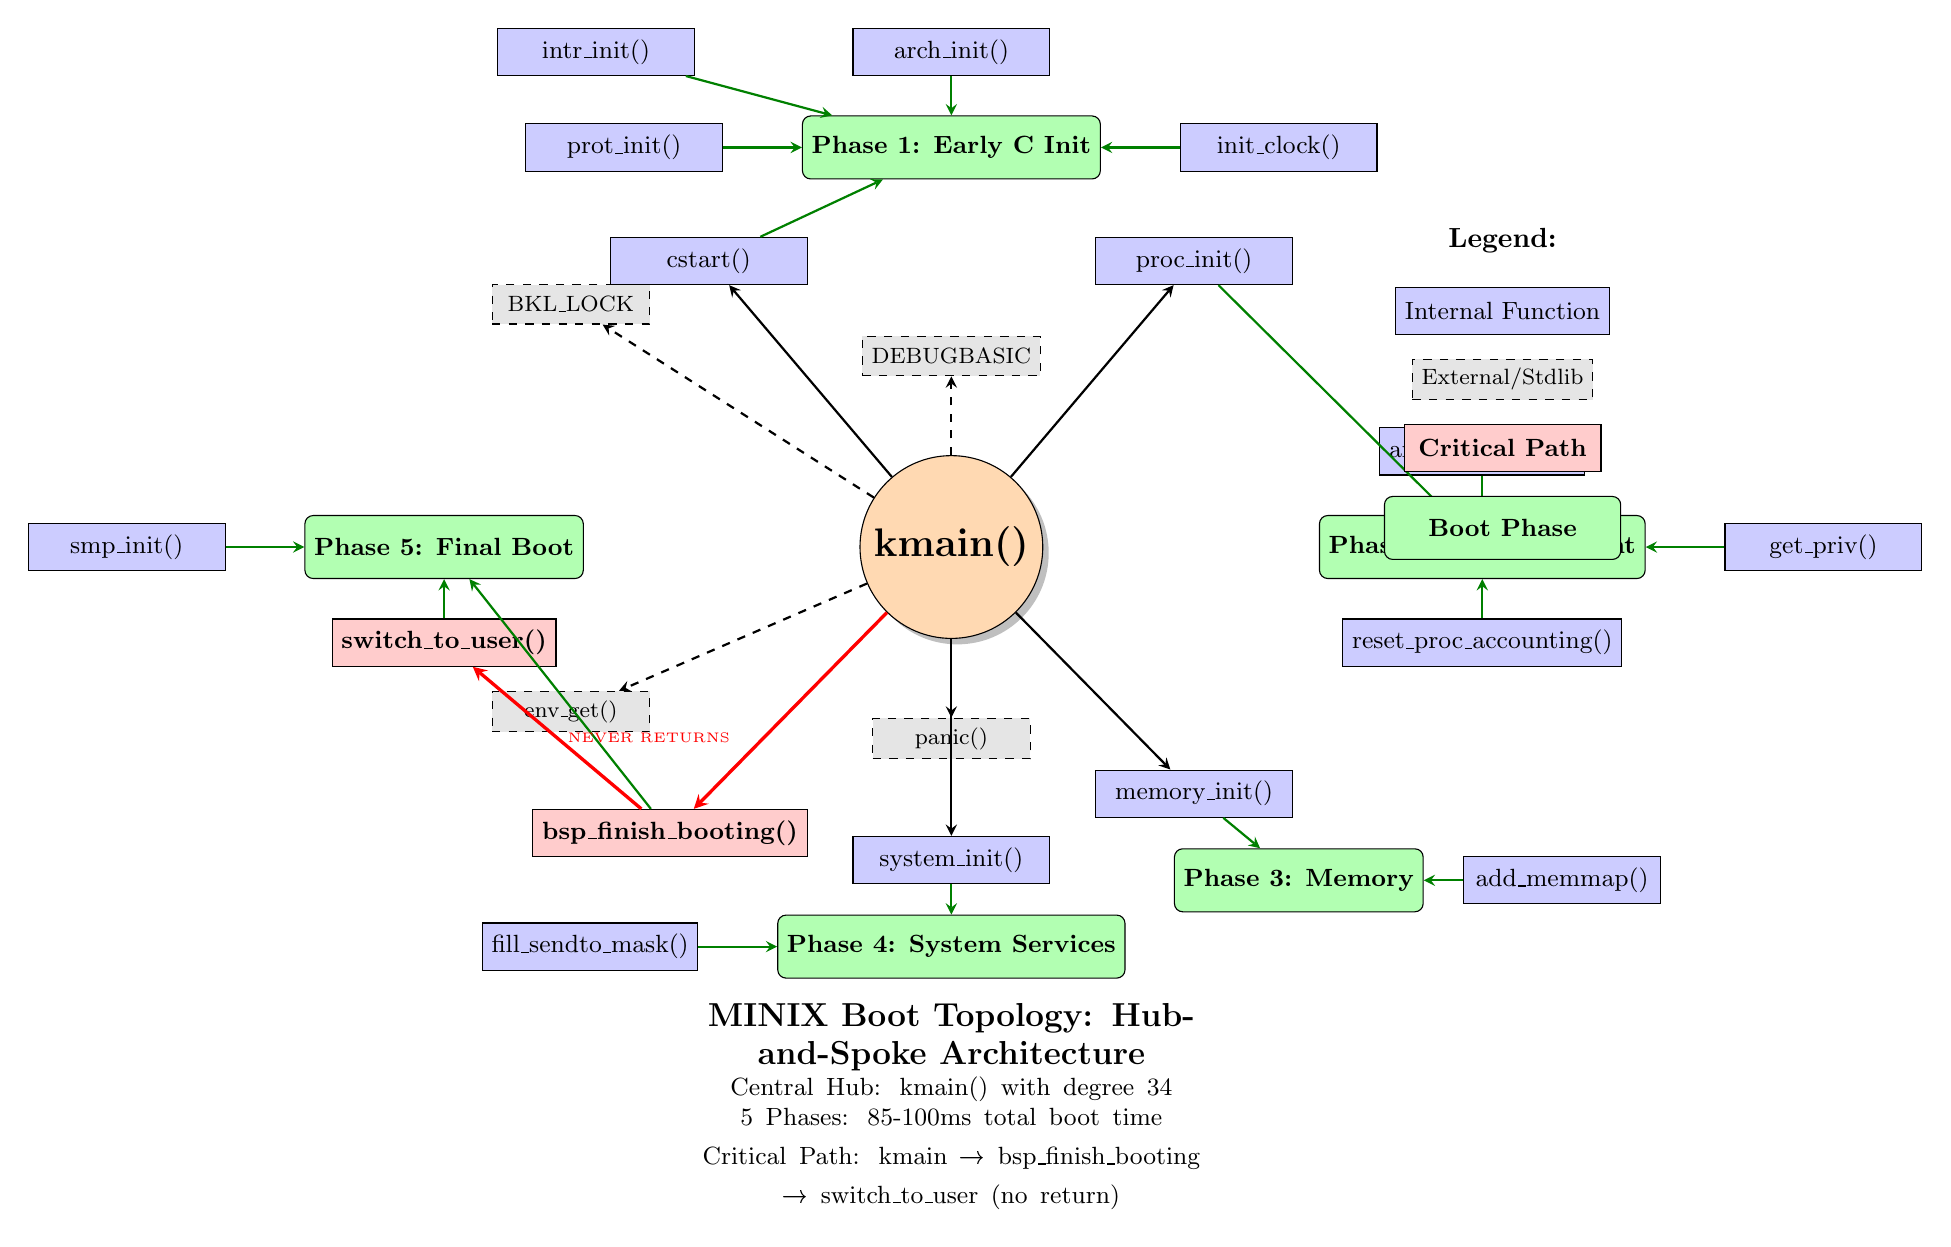
\begin{tikzpicture}[
    hub/.style={circle,draw,fill=orange!30,minimum size=2cm,font=\Large\bfseries,drop shadow},
    phase/.style={rectangle,draw,fill=green!30,minimum width=3cm,minimum height=0.8cm,rounded corners=3pt,font=\small\bfseries},
    spoke/.style={rectangle,draw,fill=blue!20,minimum width=2.5cm,minimum height=0.6cm,font=\small},
    external/.style={rectangle,draw,fill=gray!20,minimum width=2cm,minimum height=0.5cm,font=\footnotesize,dashed},
    critical/.style={rectangle,draw,fill=red!20,minimum width=2.5cm,minimum height=0.6cm,font=\small\bfseries},
    arrow/.style={->,>=stealth,thick},
    criticalarrow/.style={->,>=stealth,very thick,red},
    phasearrow/.style={->,>=stealth,thick,green!50!black},
    edge label/.style={midway,font=\tiny}
]

% Central hub
\node[hub] (kmain) {kmain()};

% Phase 1 - Early C Init (top)
\node[phase,above=3.5cm of kmain] (phase1) {Phase 1: Early C Init};
\node[spoke,above left=2.5cm and 1cm of kmain] (cstart) {cstart()};
\node[spoke,left=1cm of phase1] (prot_init) {prot\_init()};
\node[spoke,right=1cm of phase1] (init_clock) {init\_clock()};
\node[spoke,above=0.5cm of phase1] (arch_init) {arch\_init()};
\node[spoke,left=2cm of arch_init] (intr_init) {intr\_init()};

% Phase 2 - Process Management (right)
\node[phase,right=3.5cm of kmain] (phase2) {Phase 2: Process Mgmt};
\node[spoke,above right=2.5cm and 1cm of kmain] (proc_init) {proc\_init()};
\node[spoke,above=0.5cm of phase2] (arch_boot_proc) {arch\_boot\_proc()};
\node[spoke,below=0.5cm of phase2] (reset_proc) {reset\_proc\_accounting()};
\node[spoke,right=1cm of phase2] (get_priv) {get\_priv()};

% Phase 3 - Memory (bottom right)
\node[phase,below right=3cm and 2cm of kmain] (phase3) {Phase 3: Memory};
\node[spoke,below right=2cm and 1cm of kmain] (memory_init) {memory\_init()};
\node[spoke,right=0.5cm of phase3] (add_memmap) {add\_memmap()};

% Phase 4 - System Services (bottom)
\node[phase,below=3.5cm of kmain] (phase4) {Phase 4: System Services};
\node[spoke,below=2.5cm of kmain] (system_init) {system\_init()};
\node[spoke,left=1cm of phase4] (fill_sendto) {fill\_sendto\_mask()};

% Phase 5 - Final Boot (left)
\node[phase,left=3.5cm of kmain] (phase5) {Phase 5: Final Boot};
\node[critical,below left=2.5cm and 1cm of kmain] (bsp_finish) {bsp\_finish\_booting()};
\node[critical,below=0.5cm of phase5] (switch_to_user) {switch\_to\_user()};
\node[spoke,left=1cm of phase5] (smp_init) {smp\_init()};

% External/Stdlib functions
\node[external,above left=2cm and 3cm of kmain] (BKL_LOCK) {BKL\_LOCK};
\node[external,above=1cm of kmain] (DEBUGBASIC) {DEBUGBASIC};
\node[external,below left=1cm and 3cm of kmain] (env_get) {env\_get()};
\node[external,below=1cm of kmain] (panic) {panic()};

% Draw arrows from kmain to spokes
\draw[arrow] (kmain) -- (cstart);
\draw[arrow] (kmain) -- (proc_init);
\draw[arrow] (kmain) -- (memory_init);
\draw[arrow] (kmain) -- (system_init);
\draw[criticalarrow] (kmain) -- (bsp_finish);
\draw[arrow,dashed] (kmain) -- (BKL_LOCK);
\draw[arrow,dashed] (kmain) -- (DEBUGBASIC);
\draw[arrow,dashed] (kmain) -- (env_get);
\draw[arrow,dashed] (kmain) -- (panic);

% Draw phase arrows
\draw[phasearrow] (cstart) -- (phase1);
\draw[phasearrow] (prot_init) -- (phase1);
\draw[phasearrow] (init_clock) -- (phase1);
\draw[phasearrow] (arch_init) -- (phase1);
\draw[phasearrow] (intr_init) -- (phase1);

\draw[phasearrow] (proc_init) -- (phase2);
\draw[phasearrow] (arch_boot_proc) -- (phase2);
\draw[phasearrow] (reset_proc) -- (phase2);
\draw[phasearrow] (get_priv) -- (phase2);

\draw[phasearrow] (memory_init) -- (phase3);
\draw[phasearrow] (add_memmap) -- (phase3);

\draw[phasearrow] (system_init) -- (phase4);
\draw[phasearrow] (fill_sendto) -- (phase4);

\draw[phasearrow] (bsp_finish) -- (phase5);
\draw[phasearrow] (switch_to_user) -- (phase5);
\draw[phasearrow] (smp_init) -- (phase5);

% Critical path arrow
\draw[criticalarrow] (bsp_finish) -- node[edge label,right] {NEVER RETURNS} (switch_to_user);

% Annotations
\node[below=4.5cm of kmain,text width=10cm,align=center,font=\large\bfseries] {
    MINIX Boot Topology: Hub-and-Spoke Architecture\\
    \normalfont\small
    Central Hub: kmain() with degree 34\\
    5 Phases: 85-100ms total boot time\\
    Critical Path: kmain → bsp\_finish\_booting → switch\_to\_user (no return)
};

% Legend
\node[spoke,xshift=7cm,yshift=3cm] (legend1) {Internal Function};
\node[external,below=0.3cm of legend1] (legend2) {External/Stdlib};
\node[critical,below=0.3cm of legend2] (legend3) {Critical Path};
\node[phase,below=0.3cm of legend3] (legend4) {Boot Phase};
\node[above=0.3cm of legend1,font=\bfseries] {Legend:};

\end{tikzpicture}
\end{document}